计算 初值为$cos(x)$的对流扩散方程$u_t = -u_x + 0.1u_{xx}$在时间$\pi$后的结果。

以512网格的$Q_2$方法结果作为精确解, 有如下误差结果,
不难发现$Q_4$方法在误差上没有明显优势

\begin{figure}[!h]
  \caption{initial function 1}
  \centering
  \subfigure[$64 grid$]{
  \begin{minipage}[t]{0.3\linewidth}
  \centering
  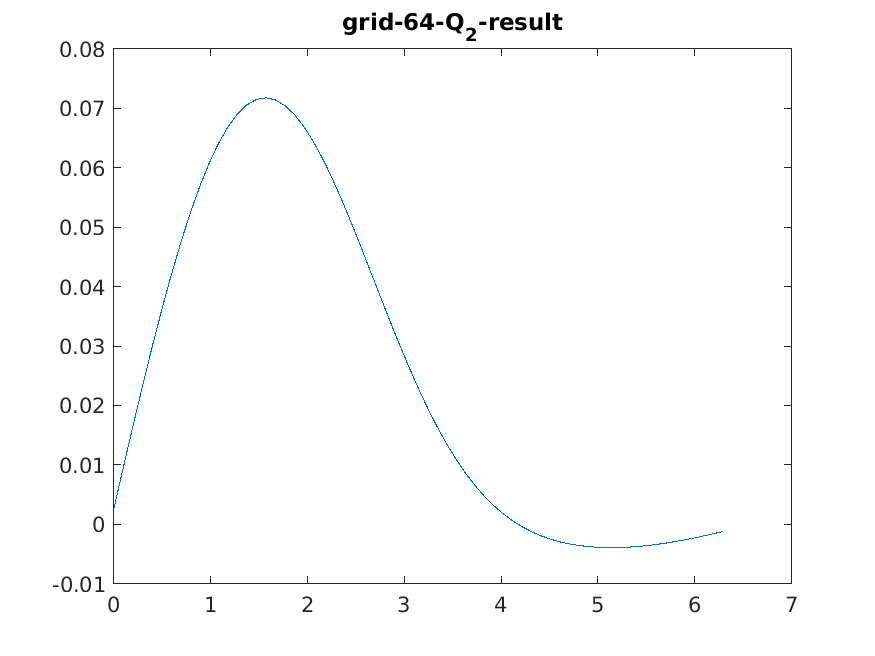
\includegraphics[height=2in, width=2in]{fig/grid-64-Q_2-result.png}
  %\caption{fig1}
  \end{minipage}%
  }%
  \subfigure[$128 grid$]{
  \begin{minipage}[t]{0.3\linewidth}
  \centering
  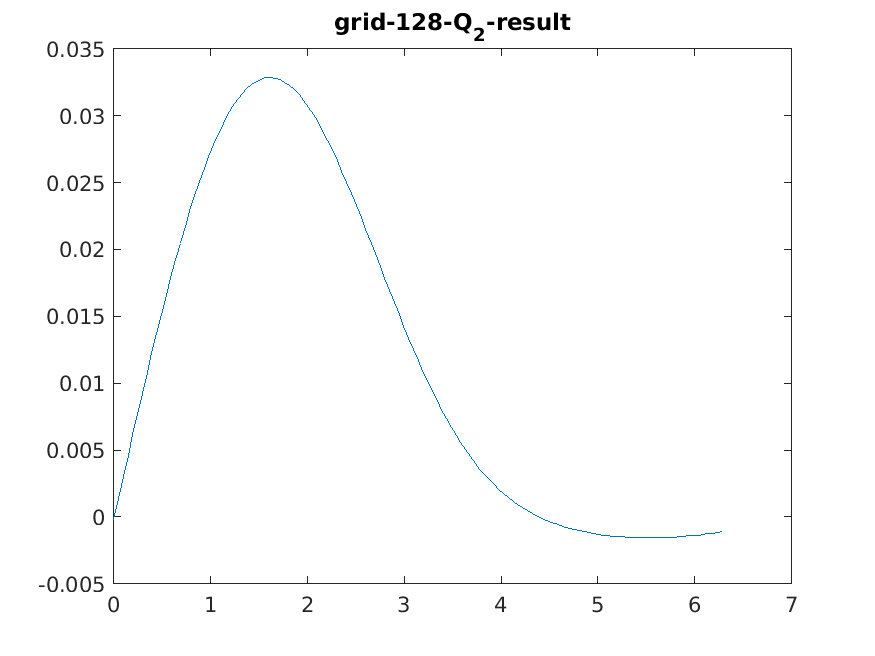
\includegraphics[height=2in, width=2in]{fig/grid-128-Q_2-result.png}
  %\caption{fig1}
  \end{minipage}%
  }%
  \subfigure[$256 gird$]{
  \begin{minipage}[t]{0.3\linewidth}
  \centering
  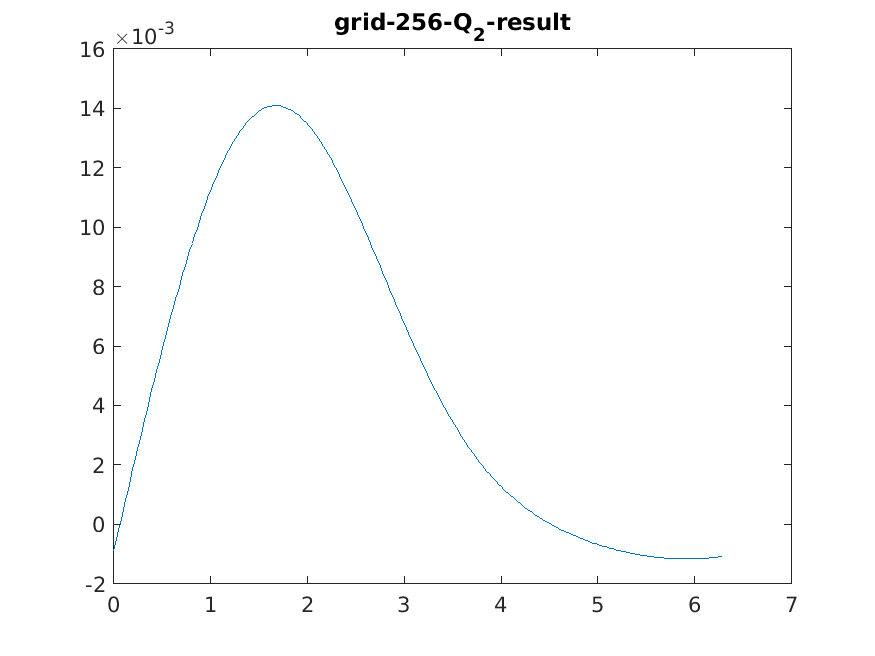
\includegraphics[height=2in, width=2in]{fig/grid-256-Q_2-result.png}
  %\caption{fig1}
  \end{minipage}%
  }%
  
\end{figure}

\begin{figure}[!h]
  \caption{initial function 2}
  \centering
  \subfigure[$Q_2$]{
  \begin{minipage}[t]{0.3\linewidth}
  \centering
  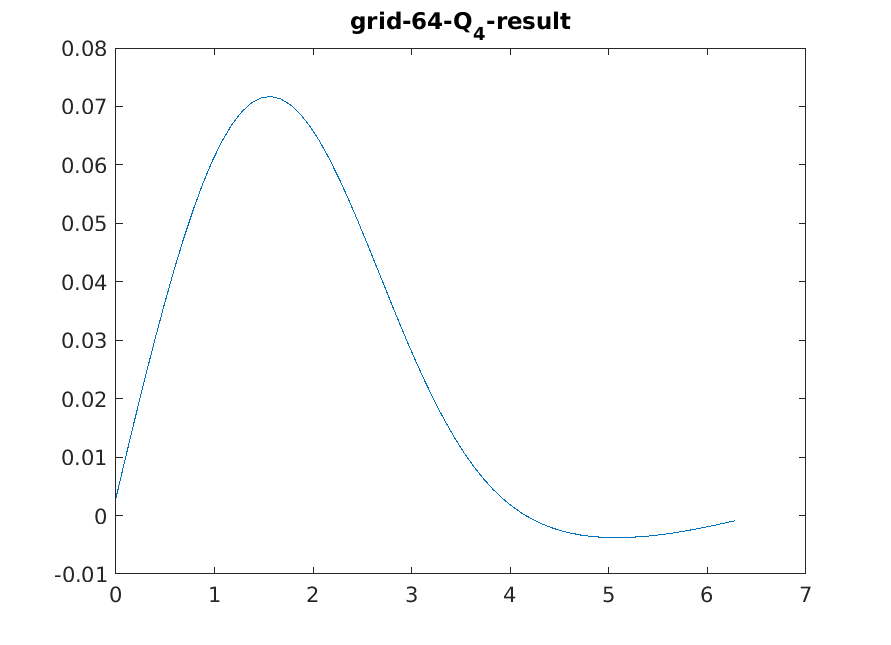
\includegraphics[height=2in, width=2in]{fig/grid-64-Q_4-result.png}
  %\caption{fig1}
  \end{minipage}%
  }%
  \subfigure[$Q_4$]{
  \begin{minipage}[t]{0.3\linewidth}
  \centering
  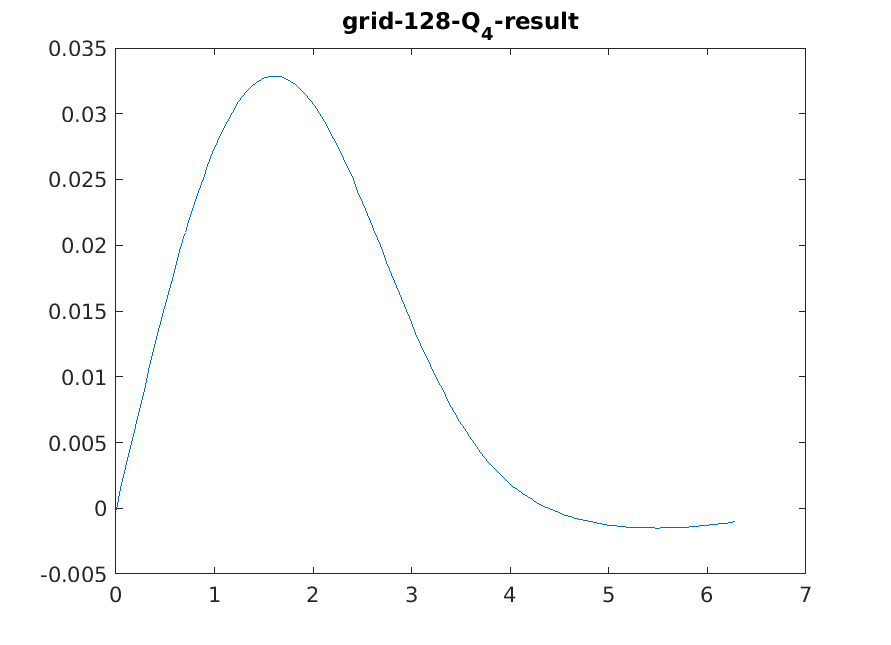
\includegraphics[height=2in, width=2in]{fig/grid-128-Q_4-result.png}
  %\caption{fig1}
  \end{minipage}%
  }%
  \subfigure[$Q_6$]{
  \begin{minipage}[t]{0.3\linewidth}
  \centering
  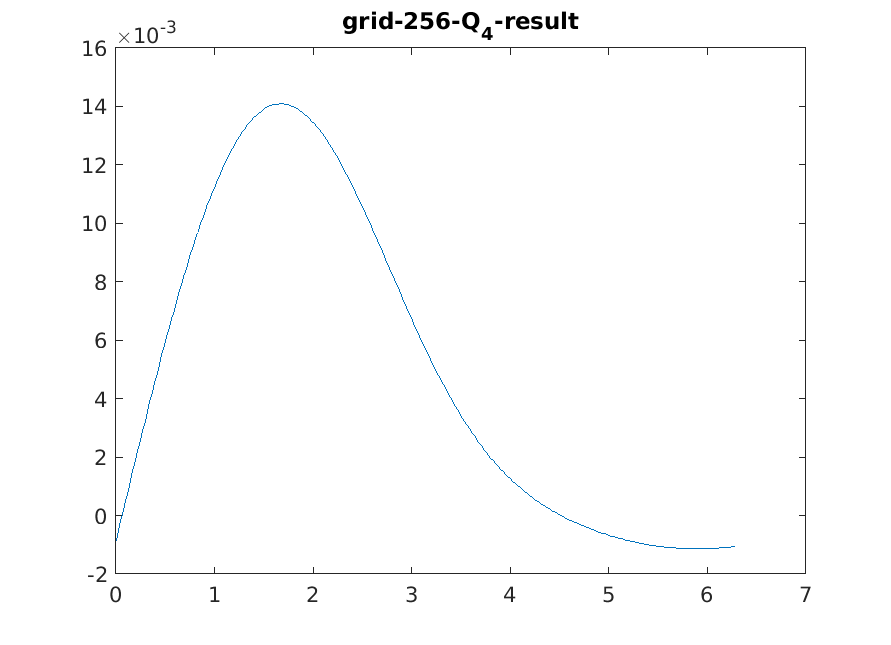
\includegraphics[height=2in, width=2in]{fig/grid-256-Q_4-result.png}
  %\caption{fig1}
  \end{minipage}%
  }%
  
\end{figure}
